\section{\texorpdfstring{Samoopravné a perfektní kody, Lloydova veta}{Samoopravné a perfektní kody, Lloydova veta}}
\vspace{5mm}
\large

\begin{definition}
	Nechť A je konečná množina (abeceda), $q = |A|$. Na množině slov $w \in A^n, |w| = n$ definujme Hammingovu metriku jako počet písmen ve kterých se liší
	\[ d_H(x, y) = |\{i : x_i \neq y_i \}| \]

	Libovolnou $C \subseteq A^n$ nazýváme kodem délky $n$ nad abecedou o $q$ symbolech. $C$ opravuje $t$ chyb, pokud
	\[ d_H(x, y) > 2t + 1 \]

	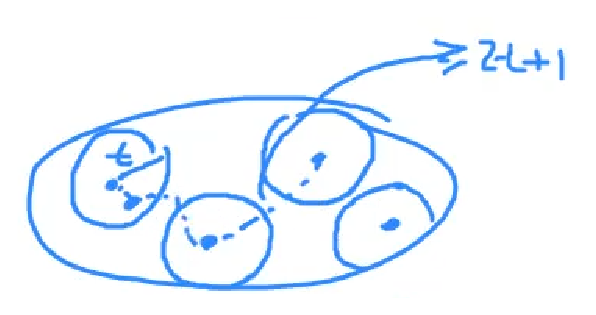
\includegraphics[scale=0.5]{code_1.eps}
\end{definition}

\begin{observation}
	Pokud vezmeme graf všech slov délky $n$, hrany povedou mezi 2 slova které se liší přesně v 1 souřadnice. Pak grafová vzdálenost je právě Hammingova metrika. Na druhou stranu tento graf je n-ta kartezská mocnina grafu o $q$ vrcholech.

	Kod $C$ opravuje $t$ chyb $\iff$ okolí kodových slov o poloměru $t$ jsou po 2 dizjunktní.
\end{observation}

\begin{observation}
	Kartezský hrana $\times$ hrana je $\square$.
\end{observation}

\begin{definition}
	\[ \Gamma(n,q) = (A^n, \{xy: d_H(x, y) = 1 \}) = K_q^n \]
\end{definition}

\begin{note}
	Pokud kod $C$ opravuje $t$ chyb, pak
	\[ |C| \leq \frac{q^n}{\sum_0^t \binom{n}{i} (q - 1)^i} \]

	Vezmeme okolí bodu $x$ poloměru $t$:
	\[ |N_{\Gamma}(x)| = 1 + n(q - 1) + ... = \]
	Kde 1 je vrchol sam, pak máme $n$ pozic na každé může dojit k $(q - 1)$ chybám.
	\[ = \frac{q^n}{\sum_0^t \binom{n}{i} (q - 1)^i} \]
	binom odpovídá způsobům zvolit písmeno. $(q - 1)^i$ je počet chyb.

	Pak nerovnice pro velikost $C$ je \# všech slov děleno velikosti okolí.

\end{note}

\begin{definition}
	Kod je t-perfektní, právě když $|C| > 1$, $C$ opravuje $t$ chyb a nastává rovnost.
	\[ |C| = \frac{q^n}{\sum_0^t \binom{n}{i} (q - 1)^i} \]

	Cely graf je pokryty okolí o poloměru $t$. Využívají beze zbytku cely graf (kodova slova).
\end{definition}

\begin{note}
	Perfektní kody skoro neexistuji.

	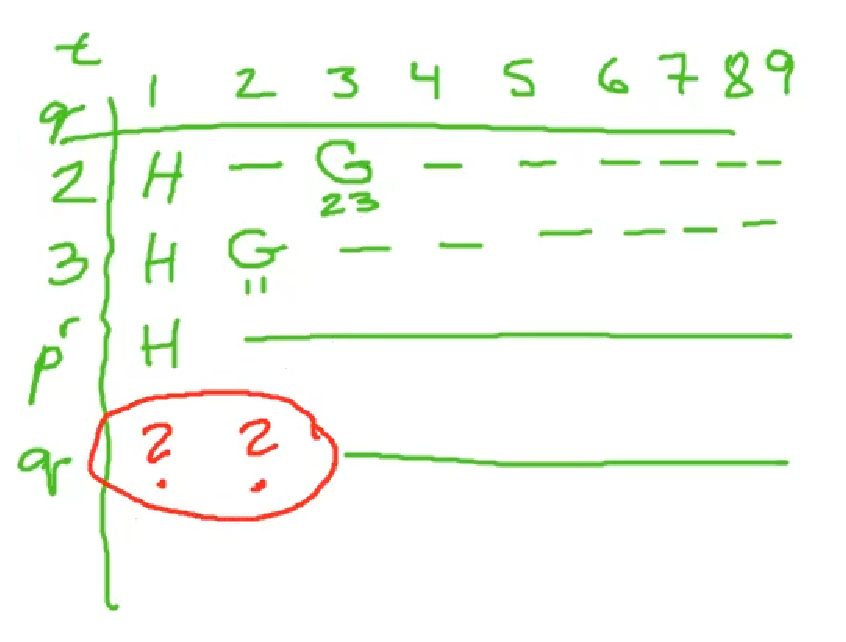
\includegraphics[scale=0.5]{code_2.eps}
\end{note}

\begin{observation}
	pro $q = p^r$, $C$ je t-perfektní kod délky $n$.
	\[ |C| = \frac{q^n}{\sum_0^t \binom{n}{i} (q - 1)^i} \in \Z \]

	Pak suma v jmenovateli dělí $q^n = p^{rm}$. Takže i suma je mocnina $p$. Dokážeme ze suma se rovna $q^l, l \in \N$.

\end{observation}

\begin{proof}
	\[ \sum_0^t \binom{n}{i} (q - 1)^i = q^a p^b = p^{ra + b}, 0 \geq b < r \]

	Upravíme sumu
	\begin{gather*}
	1 + \sum_1^t \binom{n}{i} (q - 1)^i = p^{ra + b}\\
	(q - 1)\sum_1^t \binom{n}{i} (q - 1)^{i - 1} = p^{ra + b} - 1\\
	\sum_1^t \binom{n}{i} (q - 1)^{i - 1} = \frac{q^ap^b - 1}{q - 1} = \frac{q^ap^b - p^b + p^b - 1}{q - 1} = p^b \frac{q^a - 1}{q - 1} + \frac{p^b - 1}{p^r - 1}
	\end{gather*}

	Pak $\frac{q^a - 1}{q - 1} \in \Z$ jako součet geometrické rady. Druhy zlomek ale $\in (0, 1)$. Což dává dohromady cele číslo pouze $b = 0$.
\end{proof}

\begin{theorem}[Hammingovy kody]
	Nechť $q = p^r$. Pak 1-perfektní kod délky $n$ nad abecedou o 1 symbolech existuje $\iff n = \frac{q^k - 1}{q - 1}, k \in \N$.

	Což dostaneme dosazením $t = 1$ do rovnice minulého pozorovaní:
	\[ 1 + n(q - 1) = q^k \Rightarrow n = \frac{q^k - 1}{q - 1} \]
\end{theorem}
\begin{proof}
	Nechť $C \subseteq \Z_q^n$. Sestavíme matici $H \in \Z_q^{k \times n}$ tak, aby sloupce byly po 2 lineárně nezávislé.

	V každé složce můžeme vzít $q^k$ symbolu. Nulový vektor používat nemůžeme. Dohromady $(q^k - 1)$ vektoru. Vezmeme nějaký vektor, lineárně závislé s nim jsou jeho násobky skalárem kromě 0 - $(q - 1)$. Proto
	\[ n = \frac{q^k - 1}{q - 1} \]

	Podíváme se na $Ker(H) \subseteq \Z_q^n$. Víme
	\[ \dim(Ker(H)) = n - rank(H) = n - k \]

	Tvrdíme, ze v jádru jsou vektory které mají vzdálenost aspoň 3. Pokud by existovali vektory vzdálenosti 2. Jejich rozdíl $\in Ker(H)$.
	Dostali bychom vektor $y$ který má nejvýše 2 nenulové souřadnice. Po vynásobení $Hy$ dostali bychom lineární kombinace 2 vektoru které jsou dle volby lineárně nezávislé.

	\[ |C| = q^{n - k} = \frac{q^n}{q^k} = \frac{q^n}{1 + n(q-1)} \]
\end{proof}

\begin{theorem}[Prvociselne perf. kody(BD)]
	Pro $q = p^r$ neexistuji perfektní kody jiných parametru než Hammingovy, Golayovy (a opakovací kod s parametry $q = 2, n = 2t + 1$, který je považován za triviální).
\end{theorem}

\begin{theorem}[Prvociselne perf. kody $t \geq 3$ (BD)]
	Pro $q = p^r$ neexistuji žádné t-perfektní kody opravující $t \geq 3$ chyb.
\end{theorem}

\begin{theorem}[Lloyd]
	Pokud existuje t-perfektní kod délky $n$ nad abecedou o $q$ symbolech, pak polynom:
	\[ L_t(x) = \sum_{j = 0}^t (-1)^j(q - 1)^{t - j} \binom{x - 1}{j} \binom{n - x}{t - j} \]

	má $t$ různých kladných celočíselných kořenu menších než $n$. Je to polynom stupně $t$.

	Myšlenka důkazu: najdeme 2 kořeny od sebe vzdálené min než 1. Pak nemůžou byt celočíselné.

	Pro $t = 1,2$ umíme kořeny najít, takže Lloydova veta je příliš slabá.
\end{theorem}
\begin{proof}
	TODO předn 9 od 34:00
\end{proof}

